\section{Latency Analysis}\label{latencyanalysis}
In order to understand the latency of serverless architectures in AWS Lambda services, we considered two practical use cases:
(1) Simple database applicaton
(2) Complex data analytics pipeline. We compare the latency of the serverless system with a traditional cloud VM based setup and also see how this latency is affected as the system scales to more complex architectures.

\begin{figure}[ht]
	\centering
	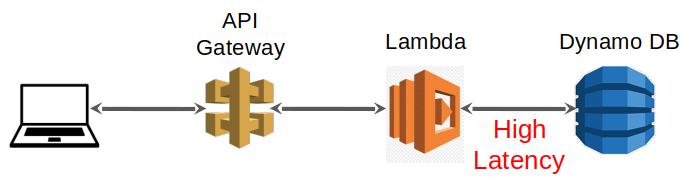
\includegraphics[width=0.7\linewidth]{image/simpleDB_serverless.png}
	\caption{Serverless for simple DB Application}\label{fig:simpleDB_serverless}
\end{figure}


\begin{figure}[ht]
	\centering
	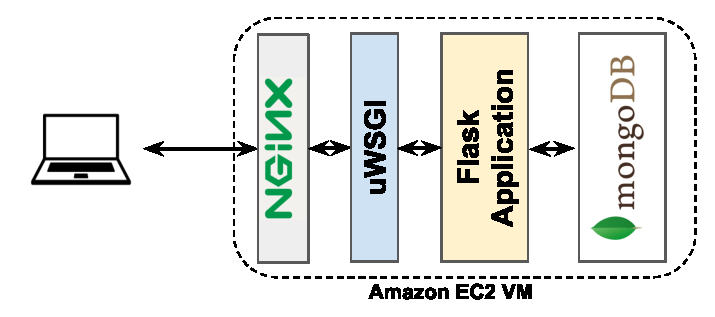
\includegraphics[width=0.7\linewidth]{image/flaskmongo.eps}
	\caption{VM based setup using Flask and MongoDB on AWS EC2}\label{fig:vmbasedsetup}
\end{figure}


\begin{figure}[ht]
	\centering
	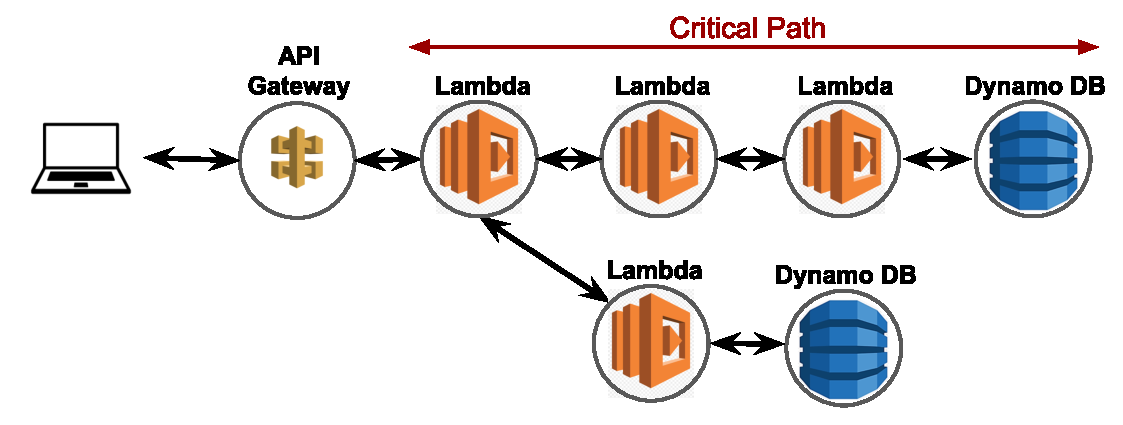
\includegraphics[width=0.8\linewidth]{image/complexserverless.eps}
	\caption{Serverless for Data analytics pipeline Application}\label{fig:DataAnalytics_serverless}
\end{figure}

\subsection{Methodology}
(1) \textbf{Simple database applicaton}: This involves only one Lambda function and one database. As the serverless functions are stateless and unlike VM we cannot save any data on it, we use Amazon's \textit{DynamoDB}\footnote{https://aws.amazon.com/dynamodb/ (Last accessed \today)}, which is a key-value and document database. In order to access the service we connect the Lambda function to an API Gateway through which it can accept HTTP requests. The architecture is depicted in Figure \ref{fig:simpleDB_serverless}. We implemented a simple application in a single lambda function using Node JS to store and retrieve account details of users from the database. In order to compare the performance of this setup relative to the traditional cloud VM based approach, we also implemented a web service with the same functionality in a VM on Amazon EC2\footnote{https://aws.amazon.com/ec2/ (Last accessed \today)} service. For this setup we used Python Flask\footnote{http://flask.palletsprojects.com (Last accessed \today)} web framework along with MongoDB as a database (Figure \ref{fig:vmbasedsetup}). The Flask application is served through Nginx\footnote{http://nginx.org/ (Last accessed \today)} web server and uWSGI\footnote{https://uwsgi-docs.readthedocs.io/en/latest/ (Last accessed \today)} application server. All these components run on the same VM with 1 vCPU and 1 GB of memory. We deployed both the  serverless and server based setups in five data centers in different regions namely, Mumbai, London, California, Canada central and Singapore. In order to make a fair comparison, to eliminate the factor of network quality delay from the end user, we only consider the time taken to process the user's request by the serverless setup and the traditional VM based setup. For serverless setup we use CloudWatch\footnote{https://aws.amazon.com/cloudwatch/ (Last accessed \today)} logs, and for server based setup we use Nginx logs to get the response time of the service.

(2) \textbf{Complex data analytics pipeline}: Here we take into account multiple lambda functions which are common for data analytics pipelines, data mining workflows, and any other complex applications involving multiple steps and processes. Any such workflow can be depicted like a graph, where the vertices are serverless components such as logic units like Lambda functions, databases like DynamoDB, file stores like Amazon S3, cache services such as Redis, etc.. There exists an edge between two such vertices if one component calls the other component and waits for its response. Or in other words, there is an edge between two components if one component depends on another component.
Thus, it is expected that the response time of the service will be equal to the sum of the computation time of the components in the longest path of the graph which is the critical path. However, since the functions and components are managed by the provider, here AWS, we do not have any control of their deployment except ensuring that they are deployed in the same region. As a result, the lambda functions, databases, and other services are deployed in different hosts and must communicate through the network which incurs some delay. This delay between each component ultimately has a severe cascading effect on the overall response time of the application. We analyzed the overall latency with different workflows of varying critical path lengths involving a series of Lambda functions terminating at DynamoDB (Figure \ref{fig:DataAnalytics_serverless}).


\subsection{Observations}

\begin{figure}[h]
	%\begin{minipage}{0.24\textwidth}
	\center
	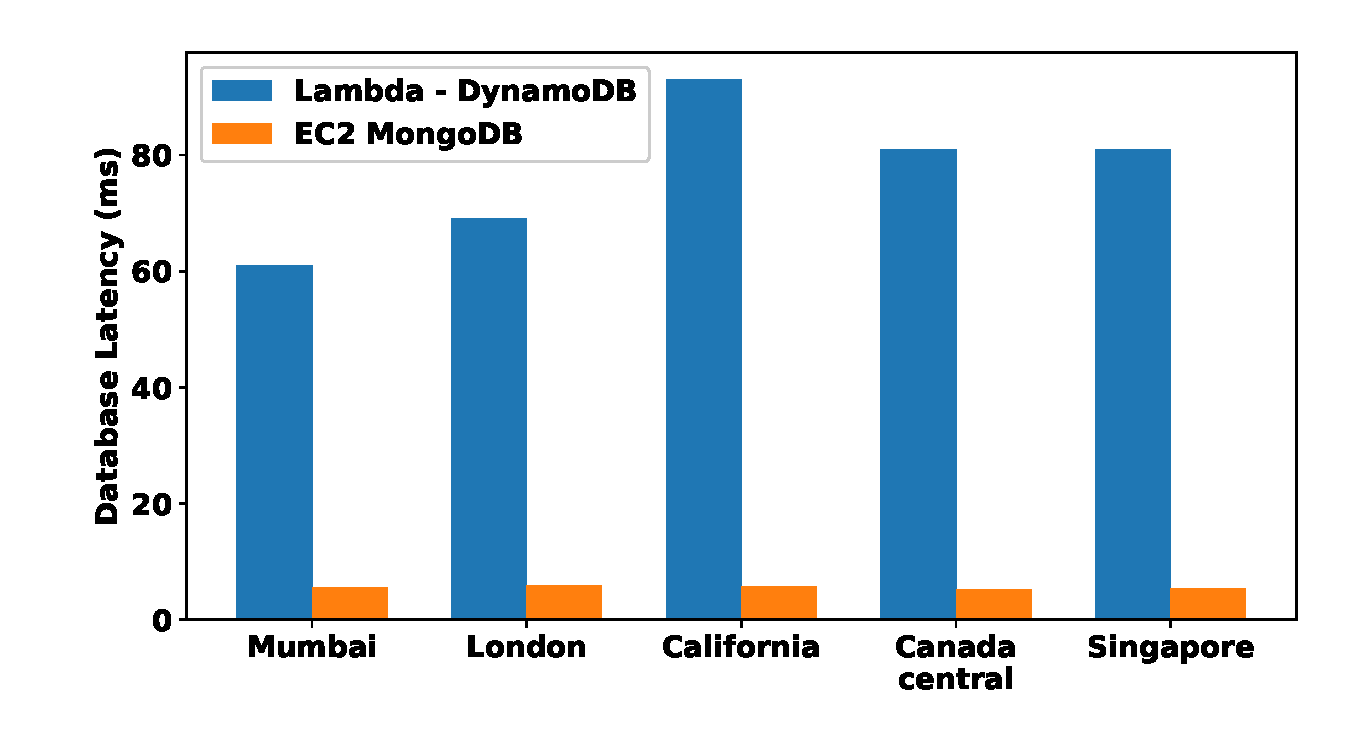
\includegraphics[width=0.9\linewidth]{image/dblatency.eps}
	\caption{DynamoDB $vs.$ MongoDb.}\label{fig:DynamoDBvsMongoDb}
	%\end{minipage}
\end{figure}


\begin{figure}[h]
	%\begin{minipage}{0.24\textwidth}
	\center
	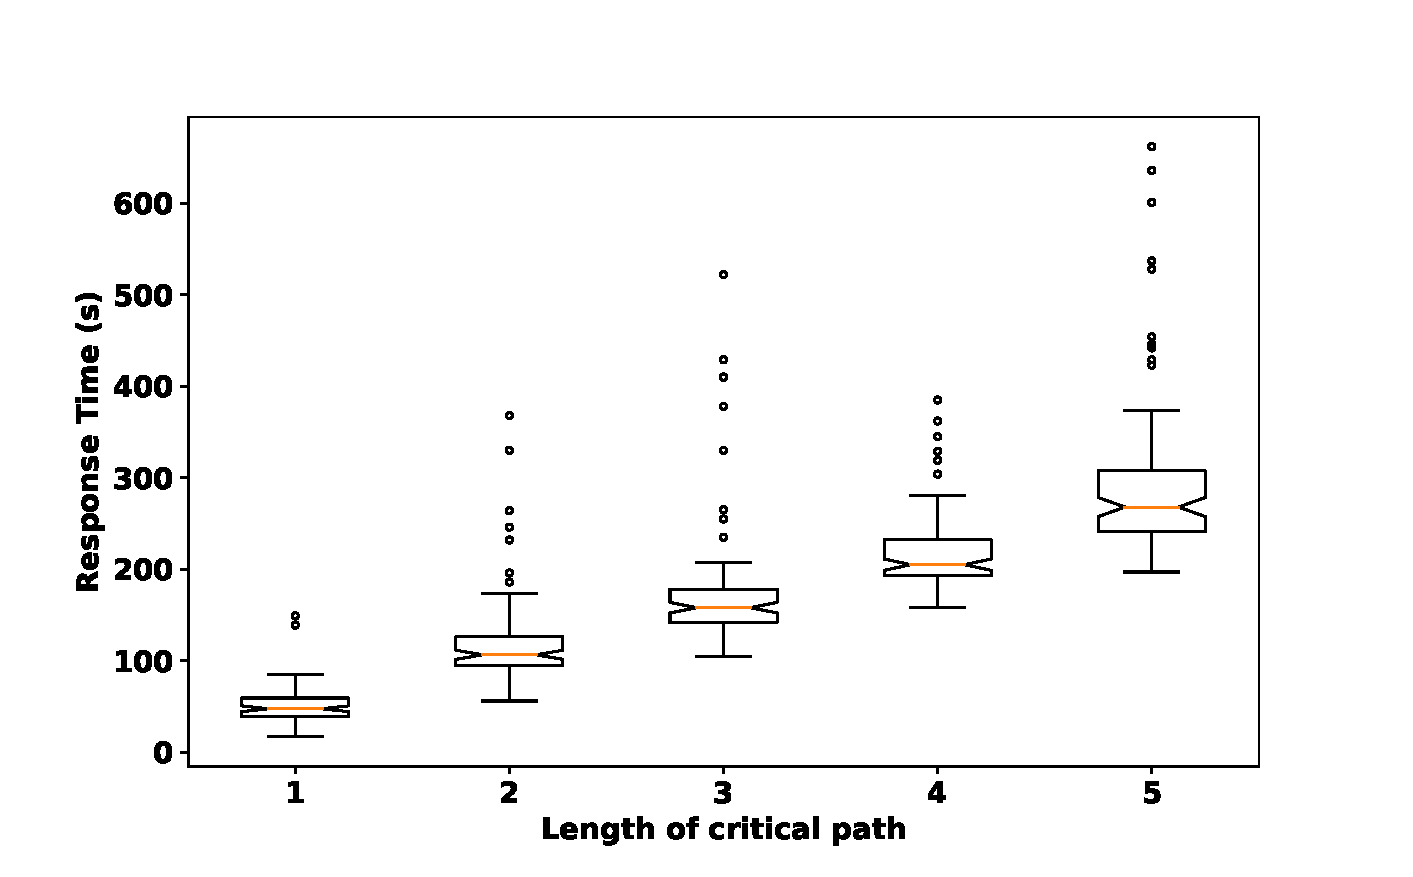
\includegraphics[width=\linewidth]{image/cascadinglatency.eps}
	\caption{serverless Cascading Data.}\label{fig:serverlessCascadingData.png}
	%\end{minipage}
\end{figure}



For the simple database application involving only a single database read or write operation per request, we measure the response time of the system per user request. We deployed both the serverless setup and the VM based setup in five regions. We observed that the  response time for the serverless architecture is significantly higher than the VM based setup. After a careful study we found that the reason of this higher latency is not because of higher processing time by the lambda function but mostly due to the latency of the database access.  In Figure \ref{fig:DynamoDBvsMongoDb}, we compare the mean database access times by the Lambda function and the Flask web application to the DyanamoDB and MongoDB respectively, in five regions. Clearly, in all regions the access time of the database in serverless setup is significantly higher than in case of the VM based setup. The most probable reason behind this is since in serverless the database and the Lambda function are not necessarily hosted on the same physical host, the DynamoDB access involves network latency, in contrast to MongoDB which is hosted in the same VM. Overall, the database access time in serverless architecture is nearly 14 times of that in traditional VM based architecture if the database is hosted in the same VM.

In the second scenario, we compared the latency of the serverless architectures with varying critical path length. The smallest such setup is of length $1$, which includes only one Lambda function and a database just like the first case. For the architecture of length $2$, the longest path involves two Lambda functions and one database at the end. Similarly we deployed such setups of critical path length $3$,$4$ and $5$. Each of the Lambda function has negligible computation and their individual response times are less than $5ms$. This allows us to monitor only the overhead due to the chaining of serverless components through network calls. Figure \ref{fig:serverlessCascadingData.png} shows the box and whisker plot of the distribution of response time for 100 user requests. We can observe that the response time of the system increases steadily with increasing length of the architecture. The mean latency of the system increases by 7.6 times from $50ms$ in case of length 1 to $430ms$ for length 5. Thus, as the serverless architectures grow more and more complex, it incurs more and more latency overhead.


\section{Serverless Caching}\label{caching}
In both the scenarios, the overall latency is a result of the network delay in between the components of the architecture. Often, this network calls can be completely avoided by caching previously computed results. However, unlike in traditional cloud VMs, in Lambda functions there is no provision to install an in-memory cache service such as Memcache, Redis etc.. Each of the requests it receives are treated separately and processed separately. AWS provides separate services such as Redis and Memcache through \textit{Amazon ElastiCache}. But although using it will avoid computational time, since they are not in the same container or host as the other components, they also have the overhead of network calls.
In order to reduce the latency futher by avoiding any network calls, we propose a memory caching technique by leveraging the Lambda container's presistency across multiple consecutive requests in short invervals and Javascript's asynchronous function calls for lazy cache updates.

\begin{figure}[h]
	%\begin{minipage}{0.24\textwidth}
	\center
	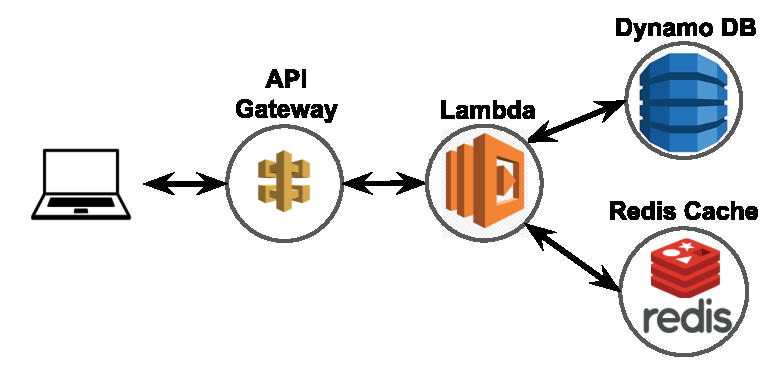
\includegraphics[width=0.8\linewidth]{image/rediscache.eps}
	\caption{Redis as a cache}\label{fig:rediscache}
	%\end{minipage}
\end{figure}


\begin{figure}[h]
	%\begin{minipage}{0.24\textwidth}
	\center
	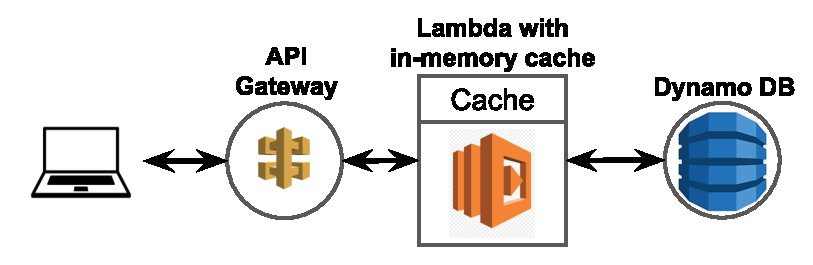
\includegraphics[width=0.8\linewidth]{image/memorycache.eps}
	\caption{In-memory cache}\label{fig:memorycache}
	%\end{minipage}
\end{figure}